% Module C: Foundations
% INStats Data Can Deceive: Causal Roadmaps with (and without) AI workshop
% August 5, 2026 | Kathryn Morrison

\documentclass[aspectratio=169]{beamer}

% Theme and packages
\usetheme{metropolis}
\usepackage[utf8]{inputenc}
\usepackage{amsmath, amssymb, mathtools, bm}
\usepackage{graphicx}
\usepackage{booktabs}
\usepackage{lmodern}
\usefonttheme{professionalfonts}
\usepackage{microtype}
\usepackage{xcolor}
\usepackage{hyperref}
\usepackage[absolute,overlay]{textpos}
\usepackage{tikz}
\usetikzlibrary{positioning,arrows.meta,shapes.geometric,calc}
\usepackage[numbers]{natbib}

\title[Foundations]{Foundations}
\subtitle{Data Can Deceive: Causal Roadmaps with (and without) AI}
\author{Kathryn Morrison}
\institute{Module C: Foundations}
\date{August 5, 2026 \quad $\cdot$ \quad 12:45--1:25 ET}

\definecolor{accent}{HTML}{4A9EFF}
\definecolor{brick}{HTML}{C0392B}
\definecolor{good}{HTML}{27AE60}
\definecolor{inkdark}{HTML}{23373B}
\setbeamercolor{structure}{fg=accent}
\setbeamercolor{background canvas}{bg=white}
\metroset{progressbar=frametitle,block=fill}
\setbeamertemplate{navigation symbols}{}
\setbeamertemplate{footline}{}

% TikZ styles for the mini-DAGs.  Node positions are held constant across
% all three graphs so that only the arrow directions change.
\tikzset{
  var/.style={circle, draw=black!70, thick, minimum size=8mm, inner sep=1pt, font=\small},
  tx/.style ={circle, draw=accent, fill=accent!12, very thick, minimum size=8mm, inner sep=1pt, font=\small},
  outc/.style={circle, draw=black!70, thick, minimum size=8mm, inner sep=1pt, font=\small},
  edge/.style={-{Stealth[length=2.2mm]}, thick},
  badj/.style={-{Stealth[length=2.2mm]}, thick, brick},
  lab/.style ={draw=black!55, rounded corners, thick, minimum height=6mm, inner sep=3pt, font=\scriptsize, align=center},
  labtx/.style={draw=accent, fill=accent!12, rounded corners, very thick, minimum height=6mm, inner sep=3pt, font=\scriptsize, align=center},
  un/.style  ={circle, draw=black!45, dashed, thick, minimum size=7mm, inner sep=1pt, font=\scriptsize},
  cond/.style={draw=brick, dash pattern=on 2pt off 1.5pt, very thick, rounded corners, minimum height=6mm, inner sep=3pt, font=\scriptsize, align=center},
  spur/.style={{Stealth[length=1.8mm]}-{Stealth[length=1.8mm]}, dashed, brick, thick},
}

\begin{document}

% ======================================================================
% Section divider
% ======================================================================
\begin{frame}[plain]
  \centering
  \vfill
  {\usebeamerfont{title}\color{inkdark}\textbf{\Large Foundations}}\\[0.6em]
  {\color{accent}\normalsize Data Can Deceive \(\cdot\) Causal Roadmaps with (and without) AI}\\[0.9em]
  {\color{inkdark}\small\textbf{Module C}}\\[0.35em]
  {\color{black!55}\small August 5, 2026}\\[0.9em]
  {\color{black!60}\small Kathryn Morrison}
  \vfill
  \begin{textblock*}{3cm}(11.9cm,0.4cm)
    
\includegraphics[width=2.6cm]{art/InStats_RWL.png}
  \end{textblock*}
\end{frame}

% ======================================================================
% Slide 2 - Association versus intervention
% ======================================================================
\begin{frame}{Association versus Intervention}
  \small
  \begin{columns}[T]
    \begin{column}{0.48\textwidth}
      \textbf{Association \;--\; \emph{seeing}}
      \begin{itemize}
        \item Patterns already in the data
        \item Treatment and outcome move together
        \item Purely descriptive: $P(Y \mid A)$
      \end{itemize}
    \end{column}
    \begin{column}{0.48\textwidth}
      \textbf{Intervention \;--\; \emph{doing}}
      \begin{itemize}
        \item What happens if \emph{we act}
        \item Outcome under a hypothetical change
        \item Requires assumptions: $P(Y \mid do(A))$
      \end{itemize}
    \end{column}
  \end{columns}
  \vspace{1em}

  \textbf{An observed association can come from:}
  \begin{itemize}
    \item a genuine causal effect,
    \item confounding (a common cause),
    \item selection, measurement, or other bias.
  \end{itemize}
  \vspace{0.6em}

  \textcolor{accent}{\textbf{The task:}} move from what we \emph{see} to what would happen if we \emph{acted}, with the assumptions made explicit.
\end{frame}


% ======================================================================
% Slide 3 - Pearl's ladder
% ======================================================================
\begin{frame}{Pearl's Ladder of Causation}
  \small
  \begin{columns}[T]
    \begin{column}{0.62\textwidth}
      \textbf{Three levels of causal reasoning} \cite{pearl2018why}:
      \vspace{0.3em}

      \begin{enumerate}
        \item \textbf{Association (Seeing)}\\
          {\footnotesize What does observing $A$ tell me about $Y$? \quad $P(Y \mid A)$}
        \item \textbf{Intervention (Doing)}\\
          {\footnotesize What happens to $Y$ if I \emph{do} $A$? \quad $P(Y \mid do(A))$}
        \item \textbf{Counterfactuals (Imagining)}\\
          {\footnotesize What \emph{would have happened} had $A$ been different?}
      \end{enumerate}
      \vspace{0.5em}

      \textcolor{accent}{\textbf{Key insight:}} each rung needs information the rung below cannot supply. No amount of observational data alone answers an interventional question.
    \end{column}
    \begin{column}{0.35\textwidth}
      \centering
      
\includegraphics[width=0.95\textwidth]{art/BoW.jpg}
    \end{column}
  \end{columns}
\end{frame}


% ======================================================================
% Slide 4 - Counterfactual contrast + fundamental problem
% ======================================================================
\begin{frame}{The Counterfactual Contrast}
  \small
  \textbf{A causal effect compares outcomes under different interventions:}
  \begin{itemize}
    \item $Y^{(1)}$: the outcome if a person \emph{were} treated, $A=1$
    \item $Y^{(0)}$: the outcome if that same person were \emph{not}, $A=0$
  \end{itemize}
  \vspace{0.5em}

  \textbf{The average causal effect is} \quad
  $E[Y^{(1)}]-E[Y^{(0)}]$ \quad (which may equal zero).
  \vspace{0.5em}

  Formalized in Hern{\'a}n \& Robins' \cite{hernan2020causal} \emph{Causal Inference: What If}.
  \vspace{0.8em}

  \begin{block}{The fundamental problem of causal inference}
    For any one person we only ever see \emph{one} of $Y^{(1)}, Y^{(0)}$.
    The other is missing, always. Causal inference is a missing-data problem
    we solve with design and assumptions, not with a bigger dataset.
  \end{block}
\end{frame}

% ======================================================================
% Slide 5 - Confounder / mediator / collider  (three DAGs, examples)
% ======================================================================
% --- Confounder ---
\begin{frame}{Confounder: A Common Cause}
  \small
  \begin{columns}[T]
    \begin{column}{0.46\textwidth}
      \centering
      \textbf{Generic structure}\\ {\scriptsize fork: \ $Z \to A$, \ \ $Z \to Y$}\\[0.9em]
      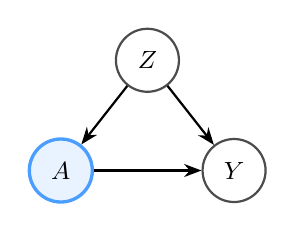
\begin{tikzpicture}
        \node[var]  (Z) at (1.1,1.4) {$Z$};
        \node[tx]   (A) at (0,0)     {$A$};
        \node[outc] (Y) at (2.2,0)   {$Y$};
        \draw[edge] (Z) -- (A);
        \draw[edge] (Z) -- (Y);
        \draw[edge] (A) -- (Y);
      \end{tikzpicture}\\[0.9em]
      \textcolor{good}{\textbf{Adjust for $Z$}} to close the backdoor.
    \end{column}
    \begin{column}{0.52\textwidth}
      \centering
      \textbf{Example: frailty}\\ {\scriptsize sicker patients get the aggressive drug}\\[0.9em]
      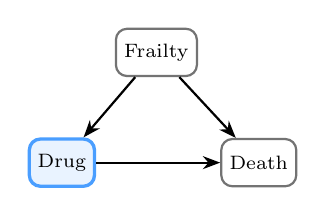
\begin{tikzpicture}
        \node[lab]   (F) at (1.2,1.4) {Frailty};
        \node[labtx] (D) at (0,0)     {Drug};
        \node[lab]   (M) at (2.5,0)   {Death};
        \draw[edge] (F) -- (D);
        \draw[edge] (F) -- (M);
        \draw[edge] (D) -- (M);
      \end{tikzpicture}\\[0.9em]
      {\scriptsize Frailty drives both treatment \emph{and} death, so the crude contrast makes the drug look harmful.}
    \end{column}
  \end{columns}
\end{frame}

% --- Mediator ---
\begin{frame}{Mediator: On the Causal Path}
  \small
  \begin{columns}[T]
    \begin{column}{0.46\textwidth}
      \centering
      \textbf{Generic structure}\\ {\scriptsize chain: \ $A \to Z \to Y$}\\[0.9em]
      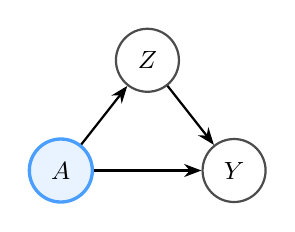
\begin{tikzpicture}
        \node[var]  (Z) at (1.1,1.4) {$Z$};
        \node[tx]   (A) at (0,0)     {$A$};
        \node[outc] (Y) at (2.2,0)   {$Y$};
        \draw[edge] (A) -- (Z);
        \draw[edge] (Z) -- (Y);
        \draw[edge] (A) -- (Y);
      \end{tikzpicture}\\[0.9em]
      \textcolor{brick}{\textbf{Do not adjust}} (for a total effect).
    \end{column}
    \begin{column}{0.52\textwidth}
      \centering
      \textbf{Example: statin and LDL}\\ {\scriptsize the drug acts \emph{through} lowering LDL}\\[0.9em]
      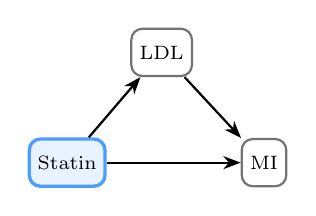
\begin{tikzpicture}
        \node[lab]   (L) at (1.2,1.4) {LDL};
        \node[labtx] (S) at (0,0)     {Statin};
        \node[lab]   (I) at (2.5,0)   {MI};
        \draw[edge] (S) -- (L);
        \draw[edge] (L) -- (I);
        \draw[edge] (S) -- (I);
      \end{tikzpicture}\\[0.9em]
      {\scriptsize Adjust for LDL and the statin looks inert -- you have removed the pathway it acts through.}
    \end{column}
  \end{columns}
\end{frame}

% --- Collider ---
\begin{frame}{Collider: A Common Effect}
  \small
  \begin{columns}[T]
    \begin{column}{0.46\textwidth}
      \centering
      \textbf{Generic structure}\\ {\scriptsize collision: \ $A \to Z \leftarrow Y$}\\[0.9em]
      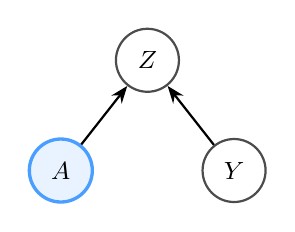
\begin{tikzpicture}
        \node[var]  (Z) at (1.1,1.4) {$Z$};
        \node[tx]   (A) at (0,0)     {$A$};
        \node[outc] (Y) at (2.2,0)   {$Y$};
        \draw[edge] (A) -- (Z);
        \draw[edge] (Y) -- (Z);
      \end{tikzpicture}\\[0.9em]
      \textcolor{brick}{\textbf{Do not adjust}} -- it opens a fake path.
    \end{column}
    \begin{column}{0.52\textwidth}
      \centering
      \textbf{Example: hospitalization}\\ {\scriptsize drug and disease both cause admission}\\[0.9em]
      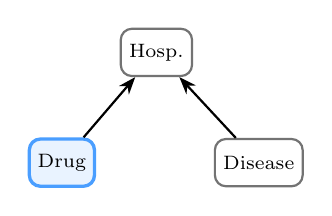
\begin{tikzpicture}
        \node[lab]   (H) at (1.2,1.4) {Hosp.};
        \node[labtx] (D) at (0,0)     {Drug};
        \node[lab]   (X) at (2.5,0)   {Disease};
        \draw[edge] (D) -- (H);
        \draw[edge] (X) -- (H);
      \end{tikzpicture}\\[0.9em]
      {\scriptsize Restrict to the hospitalized and drug and disease look linked. }
    \end{column}
  \end{columns}
\end{frame}


% ======================================================================
% Slide 6 - Why "adjust for everything" fails
% ======================================================================
\begin{frame}{Why ``Adjust for Everything'' Fails}
  \small
  A single reflex applied to all three does two kinds of damage:
  \vspace{0.6em}

  \begin{columns}[T]
    \begin{column}{0.5\textwidth}
      \textcolor{brick}{\textbf{Adjust a mediator}} \\[0.2em]
      {\footnotesize You block part of the effect you are trying to measure.
      Condition on LDL and the statin looks inert -- you have thrown away
      the mechanism.}
    \end{column}
    \begin{column}{0.5\textwidth}
      \textcolor{brick}{\textbf{Adjust a collider}} \\[0.2em]
      {\footnotesize You \emph{open} a path that was closed. Restrict to
      hospitalized patients and drug and disease look linked when in the
      population they are not.}
    \end{column}
  \end{columns}
  \vspace{1.0em}

  \textcolor{accent}{\textbf{The lesson:}} the covariate list is a set of \emph{claims about structure}, not a bigger-is-safer knob. What to adjust for is decided by the causal question and the diagram, before the data.
  \vspace{0.4em}

  {\footnotesize Which is exactly what Module D's roadmap makes systematic.}
\end{frame}

% ======================================================================
% Slide 7 - Target-trial protocol + time zero
% ======================================================================
\begin{frame}{Design First: The Target Trial}
  \small
  \textbf{Specify the randomized trial you \emph{wish} you could run} \cite{hernan2016target}, then emulate it with the data you have:
  \begin{itemize}
    \item eligibility, treatment strategies, assignment,
    \item follow-up, outcome, and the causal contrast.
  \end{itemize}
  \vspace{0.6em}

  \begin{block}{Time zero: align eligibility, treatment, and follow-up at one instant}
    Every patient's clock starts when they meet eligibility and treatment is
    assigned. Getting this wrong is the classic source of
    \textbf{immortal-time bias} (survival smuggled into the treated group)
    and \textbf{prevalent-user bias} (survivors of early treatment
    overrepresented).
  \end{block}
  \vspace{0.4em}

  \textcolor{accent}{\textbf{Why it matters here:}} a clean time zero is a \emph{design} fix for problems no downstream model can undo.
\end{frame}

% ======================================================================
% Slide 8 - Pneumonia-vaccine paradox
% ======================================================================
\begin{frame}{Why Vaccine Results Can Appear to Reverse}
  \small
  In an observational comparison, vaccinated older adults can appear to have
  \textbf{higher pneumonia risk} than unvaccinated adults.
  \vspace{0.5em}

  \textbf{A causal explanation is not the only explanation:}
  \begin{itemize}
    \item Frailer, higher-risk patients may be more likely to receive the vaccine.
    \item Frailty also raises pneumonia risk.
    \item Frailty is therefore a \textbf{confounder}: a common cause of
      vaccination and pneumonia.
  \end{itemize}
  \vspace{0.5em}

  \begin{block}{Separate real example: CAPITA}
    CAPITA was a randomized trial in adults aged 65 years or older, not the
    synthetic workshop cohort used in Modules D and F. It estimated 45.6\%
    efficacy against a first episode of vaccine-type community-acquired
    pneumonia \cite{bonten2015capita}.
  \end{block}
\end{frame}


% ======================================================================
% Slide 9 - Transition to participant checks
% ======================================================================
\begin{frame}[standout]
  Before the roadmap, test two design habits:\\[0.8em]
  classify causal roles and \textbf{align time zero}.
\end{frame}

% --- Poll 1: collider (the memorable one) ---
\begin{frame}{Poll 1 \;--\; Classify the Variable}
  \small
  Among \textbf{hospitalized} patients only, a drug's side effects and the
  underlying disease both raise the chance of admission. You analyze within
  the hospitalized group.
  \vspace{0.8em}

  Hospitalization (the variable you restricted on) is a:
  \begin{itemize}
    \item[\textbf{A.}] Confounder
    \item[\textbf{B.}] Mediator
    \item[\textbf{C.}] Collider
  \end{itemize}
\end{frame}

\begin{frame}{Poll 1 \;--\; Solution}
  \small
  \begin{columns}[T]
    \begin{column}{0.52\textwidth}
      \textcolor{good}{\textbf{C -- Collider.}}\\[0.4em]
      Side effects and disease both cause admission, so both arrows point
      \emph{into} hospitalization.\\[0.4em]
      \textcolor{brick}{\textbf{Restricting}} to it opens a fake link.
    \end{column}
    \begin{column}{0.44\textwidth}
      \centering
      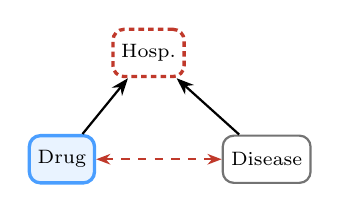
\begin{tikzpicture}
        \node[cond]  (Z) at (1.1,1.35) {Hosp.};
        \node[labtx] (A) at (0,0)   {Drug};
        \node[lab]   (Y) at (2.6,0) {Disease};
        \draw[edge] (A) -- (Z);
        \draw[edge] (Y) -- (Z);
        \draw[spur] (A) -- (Y);
      \end{tikzpicture}\\[0.3em]
      {\scriptsize\textcolor{brick}{dashed = induced association}}
    \end{column}
  \end{columns}
\end{frame}


% --- Poll 2: time-zero trap ---
\begin{frame}{Poll 2 \;--\; What Is Wrong With This Comparison?}
  \small
  Patients who filled a prescription for the drug \emph{within the first year}
  are labelled ``treated''; everyone else is ``untreated.'' Survival is
  compared from cohort entry.
  \vspace{0.8em}

  The main problem is:
  \begin{itemize}
    \item[\textbf{A.}] Too small a sample
    \item[\textbf{B.}] Immortal time -- the treated had to survive long enough to fill it
    \item[\textbf{C.}] Measurement error in the outcome
  \end{itemize}
\end{frame}

\begin{frame}{Poll 2 \;--\; Solution}
  \small
  \begin{columns}[T]
    \begin{column}{0.5\textwidth}
      \textcolor{good}{\textbf{B -- Immortal time.}}\\[0.4em]
      To be labelled ``treated,'' a patient must survive to the fill date. That
      guaranteed window biases toward the drug.\\[0.3em]
      \textcolor{accent}{\textbf{Fix:}} start time zero at treatment assignment.
    \end{column}
    \begin{column}{0.46\textwidth}
      \centering
      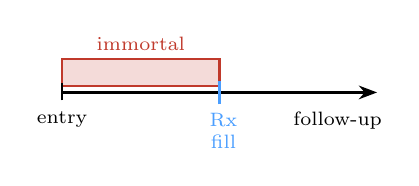
\begin{tikzpicture}[font=\scriptsize]
        \fill[brick!18] (0,0.08) rectangle (2,0.42);
        \draw[brick,thick] (0,0.08) rectangle (2,0.42);
        \node[brick] at (1,0.62) {immortal};
        \draw[thick,-{Stealth}] (0,0) -- (4,0);
        \draw[thick] (0,-0.1) -- (0,0.12); \node[below] at (0,-0.12) {entry};
        \draw[accent,very thick] (2,-0.15) -- (2,0.15);
        \node[accent,below,align=center] at (2.05,-0.14) {Rx\\fill};
        \node[below] at (3.5,-0.12) {follow-up};
      \end{tikzpicture}\\[0.5em]
      {\scriptsize survival in the shaded window is guaranteed}
    \end{column}
  \end{columns}
\end{frame}


% --- Poll 3: confounder vs mediator by timing ---
\begin{frame}{Poll 3 \;--\; Which Is Safe to Adjust For?}
  \small
  In a statin study you could adjust for LDL cholesterol measured \emph{at
  baseline}, or LDL measured \emph{at 6 months on treatment}. You want the
  \textbf{total} effect of the statin on heart attacks.
  \vspace{0.8em}

  Which is safe to adjust for?
  \begin{itemize}
    \item[\textbf{A.}] Baseline LDL
    \item[\textbf{B.}] On-treatment LDL
    \item[\textbf{C.}] Both, to be safe
  \end{itemize}
\end{frame}

\begin{frame}{Poll 3 \;--\; Solution}
  \small
  \begin{columns}[T]
    \begin{column}{0.48\textwidth}
      \textcolor{good}{\textbf{A -- baseline LDL only.}}\\[0.4em]
      \textcolor{good}{Baseline LDL} is a pre-treatment confounder (adjust).
      \textcolor{brick}{On-treatment LDL} is a mediator (do not).\\[0.3em]
      Same variable, two roles -- set by timing.
    \end{column}
    \begin{column}{0.48\textwidth}
      \centering
      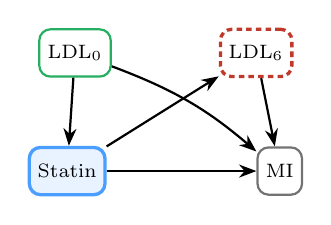
\begin{tikzpicture}[font=\scriptsize]
        \node[lab,draw=good] (L0) at (0.1,1.5) {LDL$_0$};
        \node[cond]          (L6) at (2.4,1.5) {LDL$_6$};
        \node[labtx] (A) at (0,0)   {Statin};
        \node[lab]   (Y) at (2.7,0) {MI};
        \draw[edge] (L0) -- (A);
        \draw[edge] (L0) to[bend left=10] (Y);
        \draw[edge] (A) -- (L6);
        \draw[edge] (L6) -- (Y);
        \draw[edge] (A) -- (Y);
      \end{tikzpicture}\\[0.2em]
      {\scriptsize\textcolor{good}{green=adjust}\ \ \textcolor{brick}{red=don't}}
    \end{column}
  \end{columns}
\end{frame}


% --- Poll 4: positivity ---
\begin{frame}{Poll 4 \;--\; No Comparison Group}
  \small
  Clinical guidelines mandate the drug for \emph{everyone} with severe disease,
  so in your data there are \textbf{zero untreated} severe patients.
  \vspace{0.8em}

  For the severe subgroup, you:
  \begin{itemize}
    \item[\textbf{A.}] Can still estimate the effect by adjusting
    \item[\textbf{B.}] Cannot estimate it -- there is no comparison group
    \item[\textbf{C.}] Should impute the missing untreated patients
  \end{itemize}
\end{frame}

\begin{frame}{Poll 4 \;--\; Solution}
  \small
  \begin{columns}[T]
    \begin{column}{0.5\textwidth}
      \textcolor{good}{\textbf{B -- positivity violation.}}\\[0.4em]
      Identification needs both arms within each stratum. With no untreated
      severe patients, that effect is not in the data.\\[0.2em]
      \textcolor{brick}{Imputing the arm is extrapolation.} Module D will
      formalize this as a positivity and overlap check.
    \end{column}
    \begin{column}{0.46\textwidth}
      \centering
      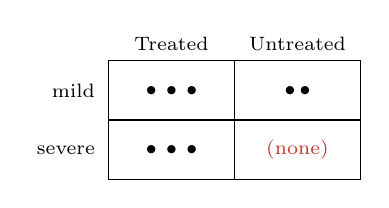
\begin{tikzpicture}[font=\scriptsize]
        \draw (0,0) rectangle (3.2,1.5);
        \draw (1.6,0) -- (1.6,1.5);
        \draw (0,0.75) -- (3.2,0.75);
        \node at (0.8,1.72) {Treated}; \node at (2.4,1.72) {Untreated};
        \node[left] at (-0.05,1.12) {mild}; \node[left] at (-0.05,0.37) {severe};
        \node at (0.8,1.12) {$\bullet\,\bullet\,\bullet$};
        \node at (2.4,1.12) {$\bullet\,\bullet$};
        \node at (0.8,0.37) {$\bullet\,\bullet\,\bullet$};
        \node[brick] at (2.4,0.37) {(none)};
      \end{tikzpicture}\\[0.3em]
      {\scriptsize no untreated severe patients = no contrast}
    \end{column}
  \end{columns}
\end{frame}


% ======================================================================
% Final handoff to Module D
% ======================================================================
\begin{frame}[standout]
  Module D turns these foundations into a reusable roadmap.\\[0.8em]
  Carry forward the target trial, time zero, DAG roles, and positivity.
\end{frame}

% ======================================================================
% Bibliography
% ======================================================================
\begin{frame}[allowframebreaks]{References}
  \tiny
  \bibliographystyle{plainnat}
  \begin{thebibliography}{9}
    \bibitem{hernan2016target}
    Hern{\'a}n MA, Robins JM.
    \newblock Using big data to emulate a target trial when a randomized trial is not available.
    \newblock \textit{American Journal of Epidemiology}, 183(8):758--764, 2016.

    \bibitem{hernan2020causal}
    Hern{\'a}n MA, Robins JM.
    \newblock \textit{Causal Inference: What If}.
    \newblock Chapman \& Hall/CRC, 2020.

    \bibitem{pearl2018why}
    Pearl J, Mackenzie D.
    \newblock \textit{The Book of Why: The New Science of Cause and Effect}.
    \newblock Basic Books, 2018.

    \bibitem{bonten2015capita}
    Bonten MJM, Huijts SM, Bolkenbaas M, et al.
    \newblock Polysaccharide conjugate vaccine against pneumococcal pneumonia in adults.
    \newblock \textit{New England Journal of Medicine}, 372(12):1114--1125, 2015.
  \end{thebibliography}
\end{frame}

\end{document}
